\documentclass{standalone}

\usepackage{circuitikz}

\begin{document}

% INT_AY22_L16_Fig02_v_a_rels.png

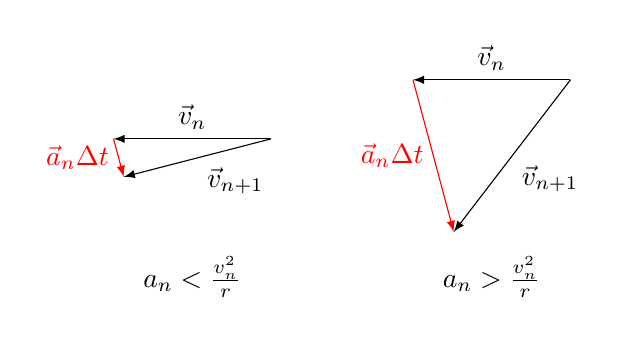
\begin{tikzpicture}[> = latex]

% Definitions

\def\R{2}

\matrix[column sep = 1 cm]{

	\begin{scope}[yshift = 0.25 cm]
		
		% Acceleration vector
		
		\draw [->, red] (180 : 2) -- node [left] {${\vec a}_n \Delta t$} ++ (-75 : 0.5) coordinate (a-end);

		% Velocity vectors
		
		\draw [->] (0, 0) -- node [above] {${\vec v}_n$} (180 : 2);
		\draw [->] (0, 0) -- node [below right] {${\vec v}_{n + 1}$} (a-end);
	
	\end{scope}
	
	% Label with accel mag
	
	\node at (-1, -1.5) {$a_n < \frac{v_n ^2}{r}$};

&

	\begin{scope}[yshift = 1 cm]
		
		% Acceleration vector
		
		\draw [->, red] (180 : 2) -- node [left] {${\vec a}_n \Delta t$} ++ (-75 : 2) coordinate (a-end);

		% Velocity vectors
		
		\draw [->] (0, 0) -- node [above] {${\vec v}_n$} (180 : 2);
		\draw [->] (0, 0) -- node [below right] {${\vec v}_{n + 1}$} (a-end);
	
	\end{scope}
	
	% Label with accel mag
	
	\node at (-1, -1.5) {$a_n > \frac{v_n ^2}{r}$};

\\
};
	
\end{tikzpicture}

\end{document}